\documentclass[twoside]{article}
\setlength{\oddsidemargin}{0.25 in}
\setlength{\evensidemargin}{-0.25 in}
\setlength{\topmargin}{-0.6 in}
\setlength{\textwidth}{6.5 in}
\setlength{\textheight}{8.5 in}
\setlength{\headsep}{0.75 in}
\setlength{\parindent}{0 in}
\setlength{\parskip}{0.1 in}

\usepackage{graphicx}
\usepackage{url}
\usepackage{wrapfig}


%
% The following commands sets up the lecnum (lecture number)
% counter and make various numbering schemes work relative
% to the lecture number.
%
\newcounter{lecnum}
\renewcommand{\thepage}{\thelecnum-\arabic{page}}
\renewcommand{\thesection}{\thelecnum.\arabic{section}}
\renewcommand{\theequation}{\thelecnum.\arabic{equation}}
\renewcommand{\thefigure}{\thelecnum.\arabic{figure}}
\renewcommand{\thetable}{\thelecnum.\arabic{table}}
\newcommand{\dnl}{\mbox{}\par}

%
% The following macro is used to generate the header.
%
\newcommand{\lecture}[4]{
  \pagestyle{myheadings}
  \thispagestyle{plain}
  \newpage
  \setcounter{lecnum}{#1}
  \setcounter{page}{1}
  \noindent
  \begin{center}
  \framebox{
     \vbox{\vspace{2mm}
   \hbox to 6.28in { {\bf COMPSCI~590S~~~Systems for Data Science
                       \hfill Fall 2017} }
      \vspace{4mm}
      \hbox to 6.28in { {\Large \hfill Lecture #1: #2  \hfill} }
      \vspace{2mm}
      \hbox to 6.28in { {\it Lecturer: #3 \hfill Scribe(s): #4} }
     \vspace{2mm}}
  }
  \end{center}
  \markboth{Lecture {#1}: #2}{Lecture {#1}: #2}
  \vspace*{4mm}
}

%
% Convention for citations is authors' initials followed by the year.
% For example, to cite a paper by Leighton and Maggs you would type
% \cite{LM89}, and to cite a paper by Strassen you would type \cite{S69}.
% (To avoid bibliography problems, for now we redefine the \cite command.)
%
\renewcommand{\cite}[1]{[#1]}

% \input{epsf}

%Use this command for a figure; it puts a figure in wherever you want it.
%usage: \fig{NUMBER}{FIGURE-SIZE}{CAPTION}{FILENAME}
\newcommand{\fig}[4]{
           \vspace{0.2 in}
           \setlength{\epsfxsize}{#2}
           \centerline{\epsfbox{#4}}
           \begin{center}
           Figure \thelecnum.#1:~#3
           \end{center}
   }

% Use these for theorems, lemmas, proofs, etc.
\newtheorem{theorem}{Theorem}[lecnum]
\newtheorem{lemma}[theorem]{Lemma}
\newtheorem{proposition}[theorem]{Proposition}
\newtheorem{claim}[theorem]{Claim}
\newtheorem{corollary}[theorem]{Corollary}
\newtheorem{definition}[theorem]{Definition}
\newenvironment{proof}{{\bf Proof:}}{\hfill\rule{2mm}{2mm}}

% Some useful equation alignment commands, borrowed from TeX
\makeatletter
\def\eqalign#1{\,\vcenter{\openup\jot\m@th
 \ialign{\strut\hfil$\displaystyle{##}$&$\displaystyle{{}##}$\hfil
     \crcr#1\crcr}}\,}
\def\eqalignno#1{\displ@y \tabskip\@centering
 \halign to\displaywidth{\hfil$\displaystyle{##}$\tabskip\z@skip
   &$\displaystyle{{}##}$\hfil\tabskip\@centering
   &\llap{$##$}\tabskip\z@skip\crcr
   #1\crcr}}
\def\leqalignno#1{\displ@y \tabskip\@centering
 \halign to\displaywidth{\hfil$\displaystyle{##}$\tabskip\z@skip
   &$\displaystyle{{}##}$\hfil\tabskip\@centering
   &\kern-\displaywidth\rlap{$##$}\tabskip\displaywidth\crcr
   #1\crcr}}
\makeatother

% **** IF YOU WANT TO DEFINE ADDITIONAL MACROS FOR YOURSELF, PUT THEM HERE:



% Some general latex examples and examples making use of the
% macros follow.

\begin{document}

%FILL IN THE RIGHT INFO.
%\lecture{**LECTURE-NUMBER**}{**DATE**}{**LECTURER**}{**SCRIBE**}
\lecture{9}{Compiled Languages: Java \& C++}{Emery Berger}{Karla Villata, Edward Pantridge}

\section{Lock Recap}
In the previous lecture locks were discussed in depth but there are a couple of points that were left out of the discussion: 

\begin{itemize}
\item  \textbf{Two Phase Locking (2PL)}  is the idea that you acquire all locks then you release all them at once. This guarantees atomicity. When dealing with deadlocks, there are two main approaches optimistic and pessimistic. The first one hopes for the "best", no deadlocks will occur while the latter one assumes the worst case scenario which is that a deadlock is bound to occur therefore to avoid it you acquire all locks. 

\item  \textbf{Avoiding deadlocks}
 If there is a cycle in locking graph, this is known as deadlock. One of the typical solutions for this is \textbf{canonical lock ordering} which means that you acquire the locks in increasing order, e.g. $lock_1$, $lock_2$, $lock_3$ and release then in decreasing order. This ensures that no cycles are form and hence is deadlock-free. 
\end{itemize}

 If you would like to read a thread of canonical lock ordering on the kernel, check out the following link. However be advised of the presence of profanity: \url{https://lkml.org/lkml/2017/10/4/580}

Going back to databases (DB), think of how would a database handle the case of getting the same commit from two different sources. Conflicts of this matter means that one of the transactions must be avoided. 

\section{Correctness Vs. Performance}
The tradeoff between high and low level programming languages is \textbf{correctness vs performance}. A high level language, is correct and easy to program at the expense of its performance. Example of high level programmig languages are:
\begin{itemize}
\item SQL
\item Haskell
\item Scala
\end{itemize}

The tradeoff of correctness is low error bound. 

\textbf{Segmentation fault SEGV } - Happens when a program write to an address that is outside of the scope of the memory that has been allocated to it. This problem is specific to low-level programs since they have access to memory. You cannot do this is Java or Scala for example.

Java is considered to be a \textit{safe language}. Defining safety in this sense is tricky but the idea is that it is considered this way because it provides safe data types and has no memory access. 

A note about SQL: SQL is so high level that is not a complete programming language. More formaly, it is not \textbf{"turing complete"}, which means that it cannot express all computations. It is common for SQL databases to extend the language to support some kind of user defined function (Java stored procedures in Orcacle, C\# user defined operations in Microsoft Server). 

\section{Java}

Java was initially an interpreted language designed to safely run in the browser. It was initially developed by Sun Microsystems \footnote{I once heard a story that the reason the famous Java IDE is named Eclipse is because they block out the sun. I am eager to hear Professor Berger confirm or deny such folklore}. The language allowed for people to write Java "Applets" which could be embedded in a web page. The applets were safe, but slow. Part of getting Applets to work correctly was achieving a portable language (aka. write once, run anywhere (WORA)). This property of Java resulted in its widespread use in servers.

Eventually Oracle bought Sun Microsystems because they wanted to add support for "stored procedures" in their databases. These are arbitrary functions written in Java that can safety be run to manipulate the database.\footnote{This is similar to User Defined Operations written in C\# for Microsoft's SQL Server.} Ever since then Oracle has been a been trying to find new ways to profit on the widespread use of Java. This includes a lawsuit with Google over the use of Java in the android operating system. To get around these legal problems, Google created their own Java Virtual Machine called Dalvik which runs a different format of Java bytecode. (I think they recently made it faster and renamed Dalvik to Android Runtime). The main difference between the JVM and Dalvik is that Dalvik is register oriented and the Oracle JVM is stack oriented.

Somewhere along the way Professor Berger got hit with two bogus cease and desist orders. One patent infringement for a memory allocator called Hoard, and one trademark infringement for another memory allocator called DieHard by the \emph{"household name"} DieHard batterys.  

\section{Java vs C++}

Despite C++ being a lower level abstraction that has the potential for better performance, the JVM is still home to many high performance projects, such as Hadoop, Spark, Clojure, Scala, and DynamoDB.

\begin{tabular}{l | l}
Java & C/C++ \\
\hline \\
JIT Compilation & AOT Compilation \\ 
Indirect access to memory & Direct access to memory (possibly unsafe)\\
Bounds checks & Explicit memory management\\
No explicit access to memory & \\
Code executes on write and read & \\
$new$ ($delete$ is handled by garbage collection. & \\
\end{tabular}

\begin{figure}[h]
\begin{center}
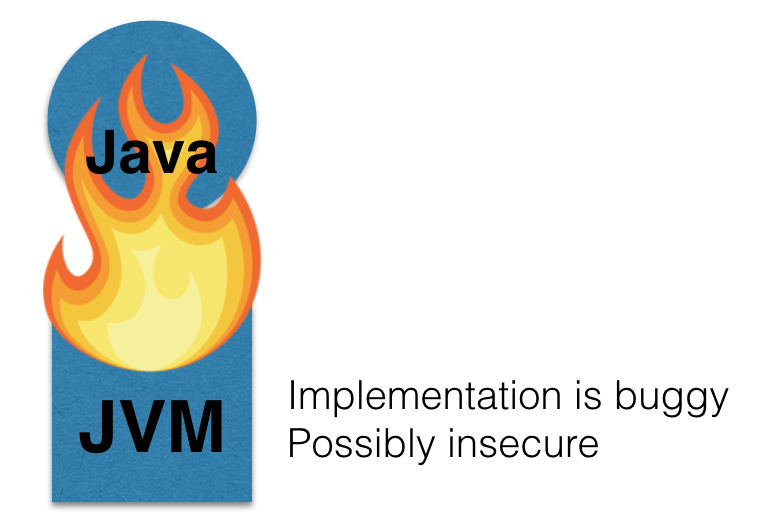
\includegraphics[width=0.4\textwidth]{fire.png}
\end{center}
\end{figure}

\subsection{JIT Compilation}

Just-In-Time. Lazy. On-demand. Designed for good throughput, but can have high latency. The reason for the high latency is a "warm-up" period where the JIT compiler is determine which code is used frequently enough to merit compilation.

This is the approach used by the JVM to compile Java bytecode to machine instructions. The JVM uses "hotspots" to find and compile code that is being used frequently.

\subsection{AOT Compilation}

Ahead-of-Time. Eager. Designed for good throughput and low latency.

This type of compilation is not possible in Java because Java is a dynamic language. In particular, Java supports things like class loaders and reflections which make AOT compilation impossible.

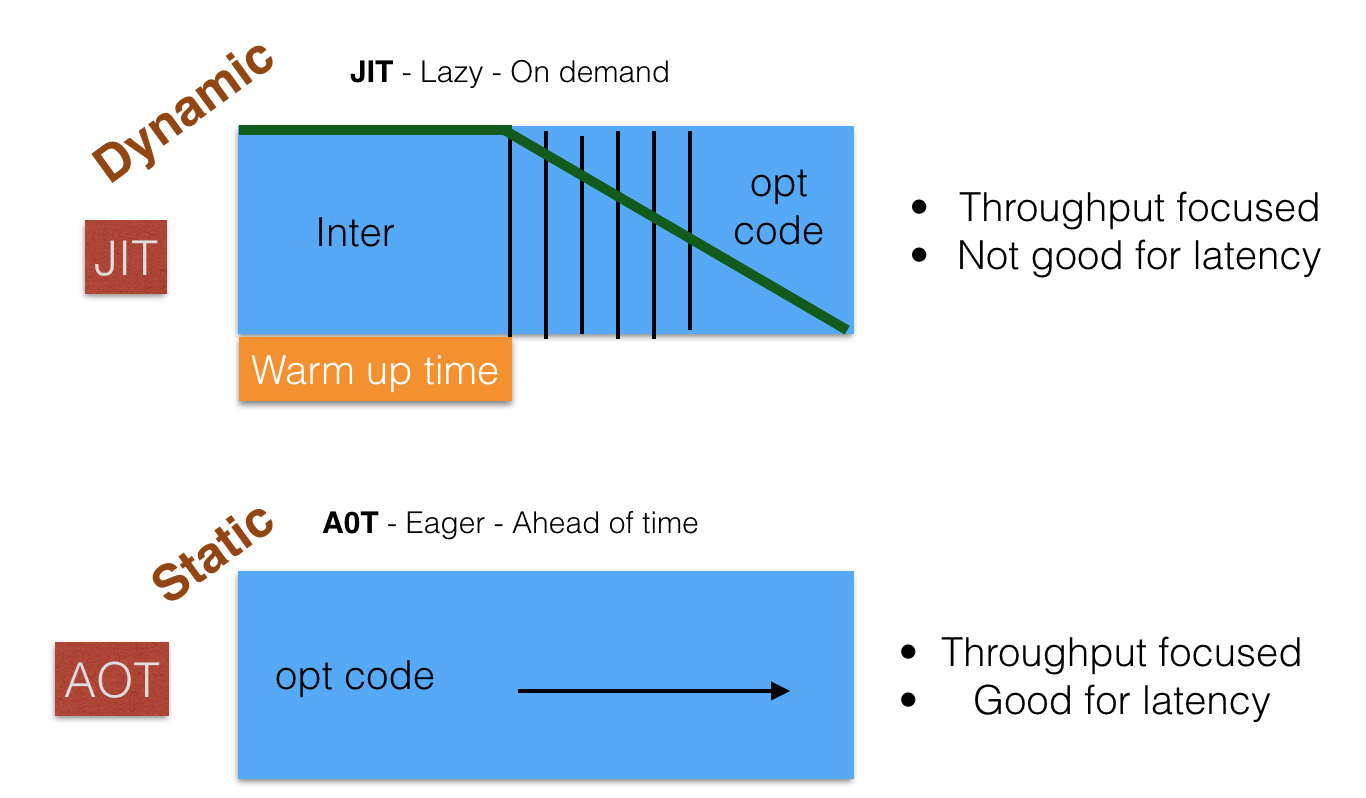
\includegraphics[width=\textwidth]{compilers.png}

\section{Compiler Optimizations}
There are different optimizations performed by compiler:

\subsection{Hoisting}

Hoisting refers to the moving of operations found in iterative control structures (ie. loops) that do not change each iteration so they are outside of the control structure. Consider the following example.

\begin{verbatim}
for (int i = 0; i < 10; i++) {
    int z = 5 + 10;
    // more logic here ...
}
\end{verbatim}

In the above code block, the variable $z$ is the same at each iteration. The compiler can "hoist" the computation of $z$ to be above the loop to avoid computing $z$ more times than necessary. The resulting computation would be equivalent to the following.

\begin{verbatim}
int z = 5 + 10;
for (int i = 0; i < 10; i++) {
    // more logic here ...
}
\end{verbatim}

\subsection{Inlining}
This refers to the task of merging in a single function functions contained within other functions. For example:

\begin{verbatim}
f() {      g() {      h() {
  A          B          C
  g();       h();     }
}          }
\end{verbatim}

This can all be combined into a single one:

\begin{verbatim}
f(){
  A
  B
  C
  D
  E
}
\end{verbatim}

The above combines all computation in a single, more efficient step. Inlining exposes optimization opportunities. If done too aggressively, it can slow down the code rather than speeding it up. 

\subsection{Constant Propagation}

Constant propagation refers to the substitution of successive assignments to the same variable with a single condensed assignment. Consider the following example of a series of statements inside a function (possibly after inlining):

\begin{verbatim}
f(){
  x = 1;       // assignment1
  x = 2;       // assignment2
  x = x + 2;   // assignment3
  x = x * x;   // assignment4
}
\end{verbatim}

It is clear that \emph{assignment1} is not necessary given that it is followed by \emph{assignment2}. Also, we can propagate the value of $x$ through assignments 3 and 4 to get a single equivalent statement. After constant propagation, the compiled definition of $f()$ would be equivalent to the following.

\begin{verbatim}
f(){
  x = 16;
}
\end{verbatim}

We also mentioned "copy propagation" as another type of compiler optimization, although we did not discuss it in depth yet.

\section{Issues with Java}

Java has a few of sources of overhead which are easier to avoid in c/c++. On average, Java is 5\% to 15\% slower than c/c++. In addition, for matrix operations Java is vastly slower than c/c++ due to Java's poor array implementation.

\subsection{Bounds Checks}

When indexing an array, the Java Virtual Machine or JVM must check that the index is within the range $\left[ 0, x\right)$ where $x$ is the length of the array. If this is not the case, then an exception is triggered. 

\subsection{Straggler Problem}

When a set of tasks is running in parallel, they must be synced at the end. If one task runs significantly longer than the others, it is considered a ``straggler''. We can think back to the Master - Worker framework. The workers refer back to the master once they all have completed their task but if one of the workers hits the garbage collector, the rest of the workers must wait for this "straggler" befored they  all get synced. This indeed slows down the pipeline since there is a high probability that at least one worker will hit the GC. 

\subsection{Space}

The garbage collection in Java has considerable memory requirements. 

\end{document}